\documentclass[12pt]{article}
\usepackage{hyperref}
\usepackage{graphicx}
\begin{document}
\title{MIT 6.882 Final Project}
\author{Jeremiah Zhe Liu,  Will Townes}
\maketitle

%\section*{Instructions} %comment out this section before turning in!
% The progress report
% (one  per  team)  will  be  a  written  pdf  document,  about  2  pages  long,
% reporting on what has been accomplished so far and outlining the work that remains to be done.
% You should write clearly about how you've spent your time so far and any preliminary  ndings
% (positive  or  negative).   Then  you  should  include  a  plan  (updated  and/or  revised  from  the  pro-
% posal,  as appropriate) for the time remaining.  If there are multiple participants,  the division of
% responsibility should be made clear.

%\newpage
\section{Dirichlet Process Sampler}
We have completed the code for sampling from the DP prior. We have also created the simulated data. We are about half-way through the Gibbs Sampler for sampling from the DP posterior. One obstacle here was we weren't sure whether to use the collapsed sampler (Chinese Restaurant Process) or a blocked sampler. It seems that Fox et al used the latter with a truncated stick-breaking process. Will worked on this part.



\section{Hierarchical Dirichlet Process Sampler}
Jeremiah worked on this part.

\section{Linear Dynamical System}
We didn't start on this part yet, although we have done some reading in the Murphy book to gain familiarity.

\section{Hidden Markov Model}
We have completed the code for generating data from HMMs. We are about half-way through the Gibbs Sampler for sampling from HMM posterior. The sampler we are using is the same as in the Fox et al paper, where we compute the backward messages and then sample from the forward conditional distributions. Will worked on this.

\section{Remaining Parts}
The hierarchical dirichlet process sampler has emerged as the most difficult component of the project. Fox et al. glossed over many complicated details for sampling from the full conditionals which we needed to dig out of supplements to other papers. However, Jeremiah has spent a lot of time working through the theory part and we anticipate making faster progress going forward. Sampling from the matrix-normal inverse wishart distribution and the linear dynamical system components are the major remaining pieces. The automatic relevance determination prior does not seem too problematic since it is just a conditionally conjugate prior. We probably will not try the Firefly MCMC approach since our data is low-dimensional.

\section{Plan and Deadlines}
Key internal deadlines are listed in parentheses.
\begin{enumerate}
\item (3/21) \\Code and visualize a dirichlet process sampler. Visualize with a simple two-dimensional clustering simulation.
\item (3/28) \\Code and visualize a``sticky'' hierarchical dirichlet process sampler. Visualize via a two-dimensional clusters-within-clusters simulation.
\item (4/4) \\Write a sampler for an ordinary (non-switching) linear dynamical system and test with simulation.
\item (4/11) \\Write a sampler for a simple hidden markov model with a fixed number of modes.
\item (4/18) \\Finish sampler from DP and HMM (Will). Finish sampler for HDP (Jeremiah). Write sampler for generative model of LDS (Will).
\item (4/25) \\Integrate HDP with HMM (Jeremiah). Integrate HMM with LDS (Will).
\item (5/2) \\Combine everything together (HDP-HMM-LDS). Prepare draft of final report.
\end{enumerate}

\newpage

\section*{Figures}

\begin{figure}
\centering
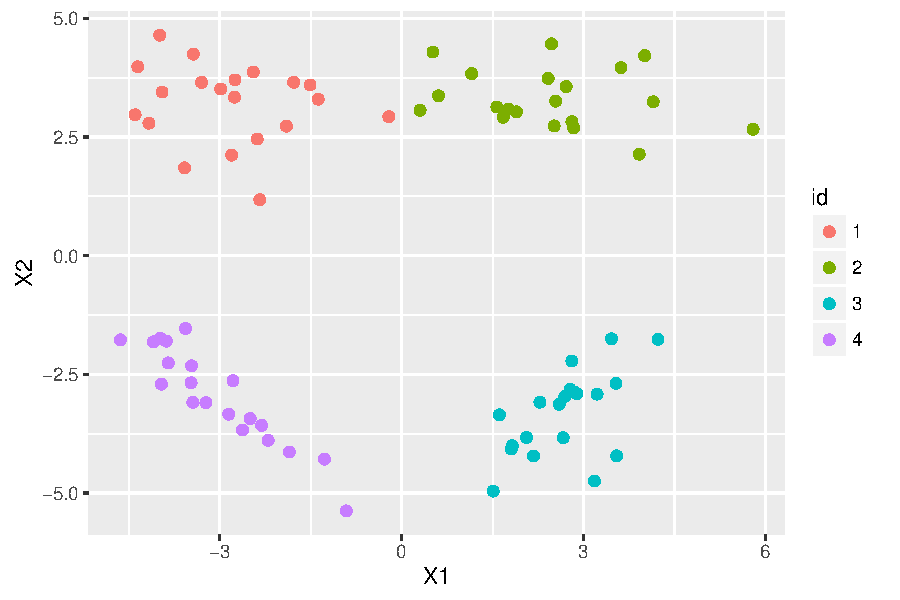
\includegraphics{plots/gmm.pdf}
\caption{Test Data for Dirichlet Process Mixture Model: A four-component Gaussian Mixture Model}
\end{figure}

\begin{figure}
\centering
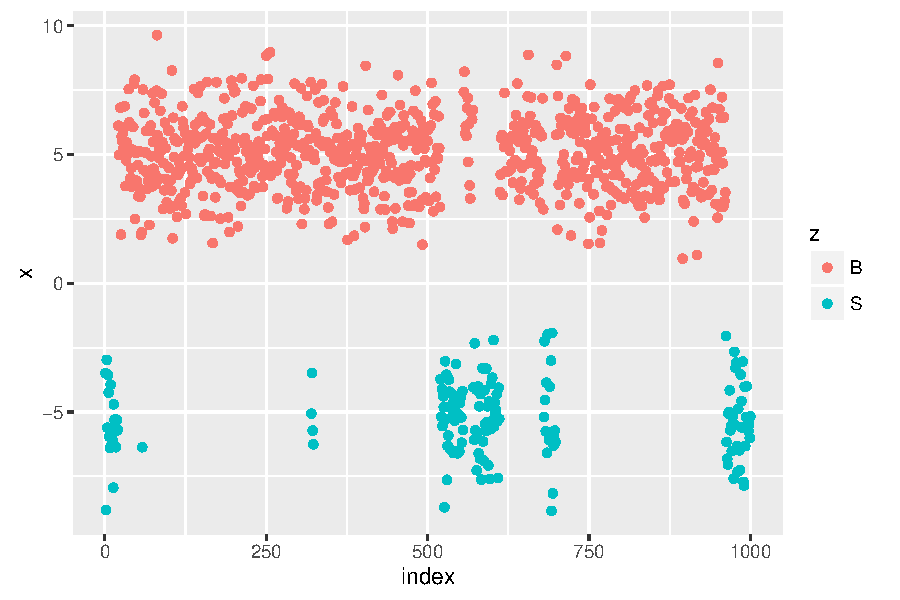
\includegraphics{plots/hmm.pdf}
\caption{Test Data for Hidden Markov Model: two hidden states with gaussian emissions}
\end{figure}

\begin{figure}
\centering
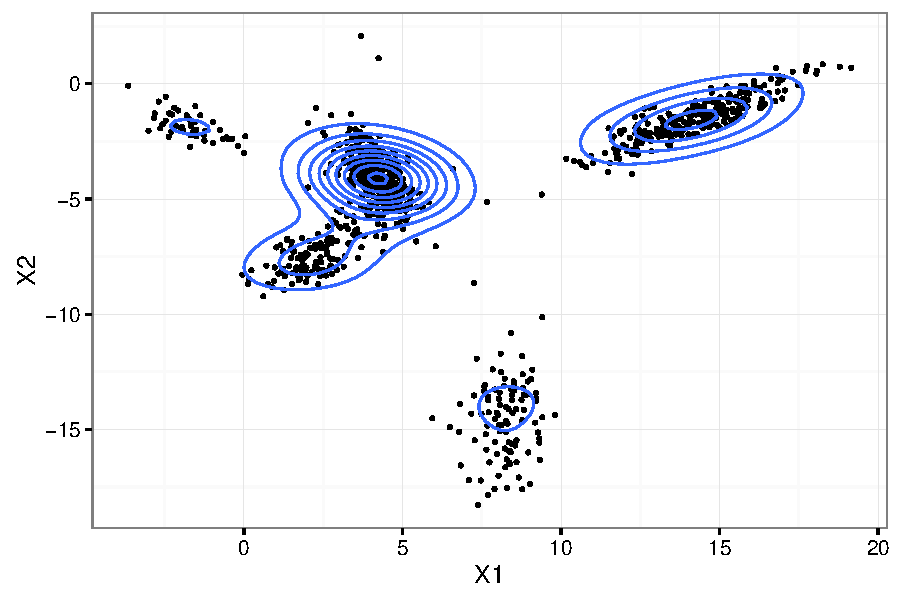
\includegraphics{plots/DP_GMM1.pdf}
\caption{Samples from DP mixture of Gaussians Prior}
\end{figure}

\begin{figure}
\centering
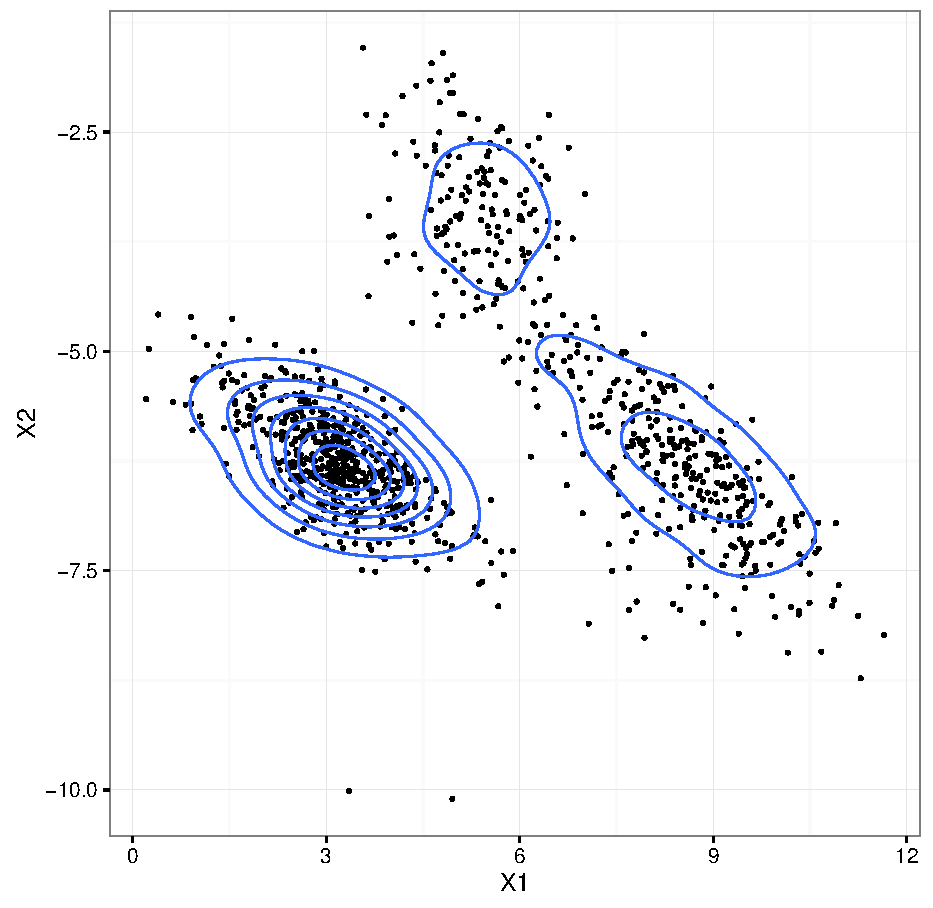
\includegraphics{plots/DP_GMM2.pdf}
\caption{Samples from DP mixture of Gaussians Prior}
\end{figure}

%\newpage
%\bibliographystyle{plain}
%\bibliography{bibliography}

\end{document}